\chapter{Typology of ${\mathbb{R}}^n$ and Fixed Point Theorems}
Typology means the "properties of subsets".

\section{Fundamental concepts}

\underline{Sets}
\begin{itemize}
    \item $\mathbb{N}$: natural numbers (1, 2, 3, ...)
    \item $\mathbb{Z}$: integers (..., -2, -1, 0, 1, 2, ...)
    \item $\mathbb{Q}$: rational numbers (fractions of integers), same as $\mathbb{Z}\cup\{\text{fractionary numbers}\}$
    \item $\mathbb{R}$: real numbers (all rational and irrational numbers), same as $\mathbb{Q}\cup\{\text{irrational numbers}\}$
    \item $\mathbb{C}$: complex numbers (numbers with real and imaginary parts), $\{a+bi, a, b\in\mathbb{R}\}$
\end{itemize}

\noindent
\underline{Symbols}
\begin{itemize}
    \item $\forall$: for all
    \item $\exists$: there exists
\end{itemize}

\noindent
\underline{Terminology}
\begin{itemize}
    \item $\in$: belongs to
    \item $\subset$: is contained
    \item $\supset$: contains
\end{itemize}

\noindent
A, B, 2 subsets of $\mathbb{R}$
\begin{itemize}
    \item $A\cup B = \{x\in\bbR:x\in A\text{ or }x\in B\}$: union of A and B, all elements in A or B
    \item $A\cap B = \{x\in\bbR:x\in A\text{ and }x\in B\}$: intersection of A and B, all elements in both A and B
    \item $A^c = \{x\in\bbR:x\notin A\}$: complement of A, all elements not in A
    \item $A\setminus B = \{x\in\bbR:x\in A\text{ and }x\notin B\}$: difference of A and B, all elements in A but not in B
    \item $\emptyset$: empty set, set with no elements
\end{itemize}

\dfn{Disjoint}{
    $A,B\subset\bbR$, A and B are disjoint iff $A\cap B=\emptyset$.
    }

\bigskip
\noindent
\underline{Properties}
\begin{itemize}
    \item Commutative: $A\cup B = B\cup A$, $A\cap B = B\cap A$
    \item Associative: $A\cup(B\cup C) = (A\cup B)\cup C$, $A\cap(B\cap C) = (A\cap B)\cap C$
    \item Distributive: $A\cup(B\cap C) = (A\cup B)\cap(A\cup C)$, $A\cap(B\cup C) = (A\cap B)\cup(A\cap C)$
    \item De Morgan's Laws: $(A\cup B)^c = A^c\cap B^c$, $(A\cap B)^c = A^c\cup B^c$
\end{itemize}

\noindent
\underline{Terminology}\bigskip\\
I is a set of indixes, $\forall_j\in I, A_j\subset\bbR$
\begin{itemize}
    \item $\displaystyle \bigcap_{j\in I} A_j = \{x\in\bbR:x\in A_j, \forall_j\in I\}$: intersection of all $A_j$, all elements in every $A_j$
    \item $\displaystyle \bigcup_{j\in I} A_j = \{x\in\bbR:x\in A_j\text{ for some }j\in I\}$: union of all $A_j$, all elements in at least one $A_j$
\end{itemize}
\ex{Union and Intersection}{
    $I_n = (-\frac{1}{n}, \frac{1}{n})$, $n\in\bbN$\\
    $\displaystyle \bigcap_{j\in\bbN} I_n= \{0\}$\\
    $\displaystyle \bigcup_{j\in\bbN} I_n= (-1,1)$
}

From now on, extending the domain where the sets live to $\bbR^n$.
$\bbR^n = \{(x_1,x_2,\cdots,x_n):x_i\in\bbR, i=1,2,\cdots,n\}$.
$\bbR^2 = \bbR\times\bbR = \{(a,b): a\in\bbR, b\in\bbR\}$.
$\bbR^n = \bbR\times\bbR\times\cdots\times\bbR = (x_1,x_2,\cdots,x_n)$.

\ex{$\bbR^2$}{
    $\bbR\times\{0\} = \{(x,0), x\in\bbR\}$, the order of the pair matters.
}

\section{Functions}

A, B sets. 
Correspondence between two sets, A and B, in such a way that to each element of A corresponds one and only one element of B.
\nt{
    element of A: objects\\elements of B that receives arrow: image\\
    $f: \underbrace{A}_{\textit{domain}}\to \underbrace{B}_{\textit{codomain}}\Rightarrow x\to\underbrace{f (x)}_{\textit{analytical expression}}$
}

\ex{Domain-1}{
    $f: D_f\to\bbR\Rightarrow x\to\sqrt{x}$\\
    $D_f = [0,+\infty)$ or $D_f = \bbR_0^+$, also called the maximal domain
}
\ex{Domain-2}{
    $g: D_g\to\bbR\Rightarrow x\to\frac{1}{x}$\\
    $D_g = (-\infty,0)\cup(0,+\infty)$ or $D_g = \bbR\setminus\{0\}$
}
\ex{Domain-3}{
    $h: D_h\to\bbR\Rightarrow x\to\ln(x)$\\
    $D_h = (0,+\infty)$ or $D_h = \bbR^+$
}
\ex{Domain-4}{
    $A\subset\bbR, l: A\to A\Rightarrow x\to x$\\
    $D_l = \bbR$, also known as the identity map
}

\dfn{Graph}{
    $f: A\to B\Rightarrow x\to f(x)$\\
Graph of f is defined as $\text{Gr}(f) = \{(x,y)\in A\times B: y=f(x)\}$.
}
\ex{Graph}{
    $f:\bbR^3\to\bbR\Rightarrow(x_1,x_2,x_3)\to x_1x_2x_3$\\
    $\text{Gr}(f) = \{(x_1,x_2,x_3,y)\in\bbR^3\times\bbR: y=f(x_1,x_2,x_3)=x_1x_2x_3\}$
}

\bigskip
\noindent
$f: A\to B\text{ where } A,B\subset\bbR$
\dfn{Injective}{
    $f(x_1)=f(x_2)\Leftrightarrow x_1=x_2$
}
An injective function, also known as one-to-one function,
is a function where distinct elements in the domain map to distinct elements in the codomain.
This means that no two different inputs can produce the same output.
\ex{Injective?}{
    $f:\bbR\to\bbR\Rightarrow x\to x^2$\\
    This is not injective because $f(1)=f(-1)=1$ but $1\neq -1$.\\
    But, if we restrict the domain to $\bbR_0^+$, then it is injective.
}
\dfnc{Surjective}{
    $\text{Image}(f) = B$
}
A surjective function, also known as onto function,
is a function where every element in the codomain has at least one element from the domain mapping to it.
This means that the function covers the entire codomain.
\ex{Surjective?}{
    $f:\bbR\to\bbR\Rightarrow x\to x^2$\\
    This is not surjective because there is no $x\in\bbR$ such that $f(x)=-1$.\\
    But, if we restrict the codomain to $\bbR_0^+$, then it is surjective.
}
\dfn{Bijective}{
    $f$ is bijective iff it is injective and surjective.
}

\bigskip
\noindent
\underline{Compontion of maps}\bigskip\\
$A,B,C\subset\bbR$,
and $\begin{cases}
    f:A\to B\\
    g:B\to C
\end{cases}$
Then, the composition of f and g is defined as $g\circ f: A\to C\Rightarrow x\to g(f(x))$.
The map is well defined if $\text{Image}(f)\subset D_g$.
\ex{Composition of maps}{
    $f:\bbR\to\bbR\Rightarrow x\to x^2$\\
    $g:\bbR\to\bbR\Rightarrow x\to x+1$\\
    $g\circ f:\bbR\to\bbR\Rightarrow x\to g(f(x))=x^2+1$\\
    $f\circ g:\bbR\to\bbR\Rightarrow x\to f(g(x))=(x+1)^2=x^2+2x+1$
}
\noindent In general, $g\circ f\neq f\circ g$ unless linear.

\dfn{Inverse}{
    f, g are maps.
    If $f\circ g = g\circ f = I_d$, then f and g are inverses of each other,
    denoted as $f = g^{-1}$ and $g = f^{-1}$,
    one with respect to other.
}
\ex{Inverse?}{
    $g: \bbR\to\bbR^+\Rightarrow x\to \exp^x$\\
    $f: \bbR^+\to\bbR\Rightarrow x\to \ln(x)$\\
    $f\circ g = f(e^x) = \ln(e^x) = x$\\
    $g\circ f = g(\ln(x)) = e^{\ln(x)} = x$\\
    $f\circ g = g\circ f = I_d\Rightarrow$
    f and g are inverses of each other.
}
\cor{Invertibility}{
    f is invertible iff f is bijective.\\
    $f:\bbR\to\bbR$ is not bijective $\Rightarrow$ f is not invertible.
}

\bigskip
\noindent
\underline{Cardinal of sets}\bigskip\\
$\Omega\subseteq\bbR^n,n\in\bbN$
\dfnc{Finite}{
    $\Omega$ is finite if $\#\Omega\in\bbN$.\\
    There exists a bijection with $\Omega$ and $\{1,2,\cdots,n\}$ for some $n\in\bbN$.
}
\ex{Cardinality}{
    $A = \{a,b,c\}$ where $a\neq b\land b\neq c\land c\neq a$\\
    $\#A = 3$
}
And of course, $\Omega$ is infinite if it is not finite.
\nt{
    $\#\emptyset = 0$
}
\bigskip
Infinite sets can be further classified into countable and uncountable sets.
\begin{itemize}
    \item $\Omega$ is countable if there exists a bijection between $\Omega$ and $\mathbb{N}$.
    \item $\Omega$ is uncountable if it is not countable.
\end{itemize}
\nt{
    In this course, finite sets are countable sets.
}
\ex{Countable}{
    $A = \{2,4,8\}$ is finite $\Rightarrow$ A is countable.
}
\ex{Countable}{
    $B = \{4,5,6,7,\cdots\} = \{n\in\bbN:x\geq 4\}$\\
    $f: B\to\bbN\Rightarrow n\to n-3$ is a bijection $\Rightarrow B$ is countable.
}
\ex{Countable}{
    $\bbZ = \{\cdots,-3,-2,-1,0,1,2,3,\cdots\}$\\
    $f:\bbN\to\bbZ\\
    n\to\begin{cases}
        0, & n=1\\
        k, & n=2k\\
        -k, & n=2k+1
    \end{cases}$ , $k\in\bbN$, is a bijection $\Rightarrow \bbZ$ is countable.
}
\ex{Uncountable}{
    $[0,1]$ is uncountable.\\
    Proof by contradiction: assume $[0,1]$ is countable. Then, there exists a bijection $f:\bbN\to[0,1]$.
    Let $f(n) = 0.a_{n1}a_{n2}a_{n3}\cdots$ be the decimal representation of $f(n)$. Construct a number $b = 0.b_1b_2b_3\cdots$ where $b_n\neq a_{nn}$ and $b_n\in\{0,1,2,\cdots,9\}$.
    Then, $b\in[0,1]$ but $b\neq f(n)$ for all $n\in\bbN$, contradicting the assumption that f is a bijection.
    Therefore, $[0,1]$ is uncountable.
}
\cor{Countability}{$\bbR$ is uncountable.}

\section{Metric spaces}
A metric space is a set equipped with a metric, which is a function that defines a distance between any two elements in the set.
$\Omega\neq\emptyset$.
\dfn{Metric}{
    A metric or distance is a map $d:X\times X\to\bbR_0^+$ that satisfies the following properties
    \begin{itemize}
        \item (Non-negativity) $d(x,y)\geq 0$
        \item (Identity of indiscernibles) $d(x,y)=0\Leftrightarrow x=y$
        \item (Symmetry) $d(x,y)=d(y,x)$
        \item (Triangle inequality) $d(x,z)\leq d(x,y)+d(y,z),\forall x,y,z\in\Omega$
    \end{itemize}
}
\ex[]{Metric}{
    $\Omega = \bbR\\
    d(x,y) = |x-y|$ is a metric.
}
\ex[]{Metric}{
    $\Omega = \bbR^2\\
    d(x,y) = \sqrt{(x_1-y_1)^2+(x_2-y_2)^2}$ is a metric.
}
\ex[]{Metric}{
    $\Omega = \bbR^n\\
    d(x,y) = \sqrt{(x_1-y_1)^2+(x_2-y_2)^2+\cdots+(x_n-y_n)^2} = \sqrt{\sum_{i=1}^n (x_i-y_i)^2}$ is a metric.
}
The metric defined above is called the Euclidean metric or Euclidean distance.
There are also other metrics such as the Manhattan metric and the distance along the surface.
\ex[]{Manhattan distance}{
    $A\to (x_A,y_A), B\to (x_B,y_B)$\\
    $d(A,B) = |x_A-x_B| + |y_A-y_B|$
}

\dfn[]{Bounded map}{
    $(X,d)$ is a metric space, $A\subset X$.\\
    $f: A\to\bbR$ is bounded if there exists $a,b\in\bbR$ such that $a\leq f(x)\leq b,\forall x\in A$.\\
    $f: A\to X$ is bounded iff $\exists a\in X,\forall x\in A, d(f(x),a)\leq M$.
}
\ex[]{Unbounded}{
    $f(x,y) = e^{x^2+y^2},(x,y)\in\bbR$\\
    $f:\bbR^2\to\bbR$\\
    $f$ is unbounded because $\displaystyle{\lim_{x^2+y^2\to\infty}} e^{x^2+y^2} = \infty$.
}
\ex[]{Bounded}{
    $g(x,y) = e^{-x^2-y^2}, (x,y)\in\bbR$\\
    $g:\bbR^2\to\bbR$\\
    $-x^2-y^2\in\bbR_0^-\\
    0<e^{-x^2-y^2}\leq 1\\
    \therefore g$ is bounded.
}

\dfn[]{Diameter}{
    $A, B\subset X$ where $(X,d)$ is a metric space.\\
    The diameter is defined as $\text{diam}(A,B) = \sup\{d(x,y),x\in A,y\in B\}$ 
    which is the maximum distance between A and B.
}
\ex[]{Diameter}{
    $X = \bbR^2$\\
    $A = \{(x,0), x\in\bbR\}$\\
    $B = \{(x,y)\in\bbR^2: (x-4)^2+(y-4)^2\leq 1\}\\
    \text{diam}(A,B) = \infty$ because A is unbounded.
}

\dfn[]{Bounded set}{
    $A\subset X$, A is bounded if diam$(x,y)\leq M$,
    for some $M\in\bbR_0^+$, and for all $x,y\in A$.
}
\nt{
    f bounded $\neq$ A bounded. f being the map and A being the set.
}
\ex[]{Bounded?}{
    $A = \bbR^2$\\
    $f: \bbR^2\to\bbR\Rightarrow (x,y)\to e^{-x^2-y^2}$\\
    f is bounded, i.e. bounded range, but A is unbounded, i.e. unbounded domain.
}
\ex[]{Bounded?}{
    $A = [-1,1]\times[2,3]$\\
    $B = \bbR^2$\\
    $f: A\to B\Rightarrow (x,y)\to(2x,2y)$\\
    f is bounded, i.e. bounded range, and A is bounded, i.e. bounded domain.
}
\ex[]{Bounded?}{
    $A = (0,1)$\\
    $f(x) = \ln(x)$\\
    f is unbounded, i.e. unbounded range, but A is bounded, i.e. bounded domain.
}

\section{Definition and typology}
$X = \bbR^n, A\subset X, a\in A, r>0$
\dfn{Open ball}{
    An open ball centered at $a\in X$ and radius $r>0$ is defined as\\
    $B_r(a) = \{x\in X: d(a,x)<r\}$.
}
\dfn[]{Closed ball}{
    A closed ball centered at $a\in X$ and radius $r>0$ is defined as\\
    $D_r(a) = \{x\in X: d(a,x)\leq r\}$.
    D is for "disk". $D_r(a) = \overline{B_r(a)}$.
}
\dfn[]{Open set}{
    A is an open set of X iff $\forall x\in X, \exists r>0: B_r(x)\subset A$.
}
\dfn[]{Interior point}{
    $X_0$ is an interior points of A if there exists $r>0$ such that $B_r(x_0)\subset A$.\\
    We write $\text{int}A$.
}
\dfn[]{Adherent point}{
    $X_0$ is an adherent point if for all $r>0$, $B_r(x_0)\cap A\neq\emptyset$.\\
    Same notation as closure: $\overline{A}$ or $\text{cl}(A)$.
    Can also be written as $\text{ad}(A)$.
}
\dfn[]{Frontier point}{
    $X_0$ is a boundary or frontier point of A if for any $r>0$, $B_r(x_0)\cap A\neq\emptyset$
    and $B_r(x_0)\cap A^c\neq\emptyset$.\\
    We write $\text{fr}(A)$ or $\partial A$.
}
\dfn[]{Closed set}{
    $A\subset X$ is a closed set iff $A^c$ is open, $X\to\bbR^n$.
}
\ex[]{}{
    $A = [0,1]\subset\bbR\\
    \text{int}(A) = (0,1)\\
    \text{cl}(A) = [0,1]\\
    \text{fr}(A) = \{0,1\}\\
    A$ is closed but not open becasuse $A^c = (-\infty,0)\cup(1,+\infty)$ which is open.
}
\dfn[]{Exterior point}{
    $B\subset \bbR^n$ \\
    y is an exterior point of B iff $y\in\text{int}(B^c)$.
}
\ex[]{}{
    $A = [0, 1)$\\
    $A^c = (-\infty,0)\cup[1,+\infty)$\\
    $\text{int}(A^c) = (-\infty,0)\cup(1,+\infty)$\\
    $\text{ext}(A) = (-\infty,0)\cup(1,+\infty)$
}
\ex[]{}{
    $B = [0,1)\times[0,1)$\\
    $B^c = [(-\infty,0)\times\bbR]
    \cup[[0,\infty)\times\bbR^-]
    \cup[[1,\infty)\times\bbR]
    \cup[[0,1]\times[1,\infty)]$\\
}
\textbf{Proposition:} $A\subset\bbR^n$
\begin{enumerate}
    \item Any open ball is an open set.
    \item $\text{int}(A)\subset A\subset\text{cl}(A)$
    \item A is open $\Leftrightarrow$ A = int(A)
    \item A is closed $\Leftrightarrow$ A = cl(A)
    \item $\text{cl}(A) = \text{int}(A)\cup\partial A$
    \item $\partial A$ is closed.
    \item A countable union of open sets is open.
    \item A countable intersection of closed sets is closed.
\end{enumerate}
\ex[]{}{
    $A = [0,1)\cup[2,3]$
    \begin{itemize}
        \item $\text{int}(A) = (0,1)\cup(2,3)\rightarrow$ interior is always open
        \item $\text{cl}(A) = [0,1]\cup[2,3]\rightarrow$ closure is the interior and the walls
        \item $\partial A = \{0,1,2,3\}$
        \item A is open? No. Because $A\neq \text{int}(A)$
        \item A is closed? No. Because $A\neq \text{cl}(A)$
    \end{itemize}
}
\textbf{Remarks:}
\begin{enumerate}
    \item There are sets that are neither open nor closed.
    \item $\bbR^n,\emptyset$ are either open or closed.
\end{enumerate}
\ex[]{}{
    $B = \{(x,y)\in\bbR^2 : x^2+(y+2)^2\leq 4\}$\textbackslash$\{(0,0)\}$
    \begin{itemize}
        \item $\text{int}(B) = \{(x,y)\in\bbR^2 : x^2+(y+2)^2< 4\}$
        \item $\text{ext}(B) = \{(x,y)\in\bbR^2 : x^2+(y+2)^2> 4\}$
        \item $\text{cl}(B) = \{(x,y)\in\bbR^2 : x^2+(y+2)^2\leq 4\}$
        \item $\partial B = \{(x,y)\in\bbR^2 : x^2+(y+2)^2= 4\}$
        \item B is open? No. Because $B\neq \text{int}(B)$
        \item B is closed? No. Because $B\neq \text{cl}(B)$
    \end{itemize}
}
\dfn[]{Bounded}{
    $A\subset\bbR^n$\\
    A is bounded if $A\subset B_r(x_0)$, for some $r>0$ and some $x_0\in\bbR^n$.
}
\ex[]{}{
    $\bbR\times\{0\}\subset\bbR^n$\\
    Not bounded because we cannot find a $x$ large enough to contain the entire set.
}
\dfn[]{Compact}{
    $A\subset\bbR^n$\\
    A is compact iff A is closed and bounded.
}
\dfn[]{Association point}{
    $A\subset\bbR^n$\\
    $x_0$ is an association point of A if for any $r>0$, $B_r(x_0)\cap [A$\textbackslash$\{x_0\}]\neq\emptyset$
}
\ex[]{}{
    $A = \{\frac{1}{n},n\in\bbN\}\subset\bbR$\\
    $0\in A$? No. But there are points from A that accumulates in the ball of 0.\\
    $\therefore$ 0 is an accumulation point of A.
}
\dfn[]{Isolated point}{
    $A\subset\bbR^n$\\
    $x_0$ is an isolated point of A if $x_0\in A$ and $x_0$ is not an accumulation point of A.
}
\bigskip
\textbf{Proposition:}\\
$\text{cl}(A) = \text{int}(A)\cup\partial A = \{\text{accumulation points}\}\cup\{\text{isolated points}\}$, 
accumulation points can also be written as derivative of A, $A'$.\bigskip\\
\textbf{Remarks:}\\
$x^2 = 9\Leftrightarrow x = -3\lor x = 3$\\
$\{x\in\bbR : x^2 = 9\}\rightarrow$ two points\\
$\{(x,y)\in\bbR^2 : x^2 = 9\}\rightarrow$ two lines\\
$\{(x,y,z)\in\bbR^3 : x^2 = 9\}\rightarrow$ two planes\\
\dfn[]{Neighborhood}{
    $\bbR^n, x_0\in\bbR^n$\\
    $\nu$ is a neighborhood of $x_0$, if there exists $r>0$ such that $B_r(x_0)\subset \nu$.\\
    In general, we consider open neighborhood.
}
\bigskip
\textbf{Remarks:}
\begin{enumerate}
    \item $g = \frac{1}{f}$, $D_g = \{x\in\bbR^n : f(x)\neq 0\}$
    \item $g = \log(f)$, $D_g = \{x\in\bbR^n : f(x)> 0\}$
    \item $g = \sqrt{f}$, $D_g = \{x\in\bbR^n : f(x)\geq 0\}$
\end{enumerate}
\dfn[]{Convex}{
    $A\subset\bbR^n$\\
    A is convex if for any two points X and Y in A, then the segment $[X,Y]$ is contained in A.
}

\section{Sequences in $\bbR^n$}
Map from a subset of $\bbN$ into $\bbR^n$.
\ex[]{Sequence}{
    $f(n) = n^2, n\in\bbN$\\
    $f: \bbN\to\bbR\Rightarrow n\to n^2$\\
    $u_n = f(n) = n^2\rightarrow$ general term
}
\ex[]{Sequence}{
    $V_n = (n^2, n^2+1)$ is a sequence in $\bbR^2$.\\
    $V_5 = (25, 26)$
}
Sometimes, it is important to see the convergence of sequences.\\
$u_n = \frac{1}{n}$\\
$\lim_{n\to\infty} u_n = 0 \Rightarrow u_n\rightarrow0$
\lem[]{}{
    If a sequnece $u_n$ in $\bbR$ converges, the limit is unique.
}
$u_n = (a_{1n}, a_{2n}, \cdots, a_{kn})\in\bbR^k\rightarrow$ the sequence converges if each component converges.
\ex[]{Convergence}{
    $u_n = (\frac{1}{n}, \frac{n^2-2}{n^2})$ is a sequence in $\bbR^2$
    \begin{itemize}
        \item $\frac{1}{n}\rightarrow 0$
        \item $\frac{n^2-2}{n^2} = 1-\frac{2}{n^2}\rightarrow 1$
    \end{itemize}
    $\therefore u_n\rightarrow(0,1)$, $u_n$ converges.
}
When one of the components does not converge, we say that the sequence diverges.
\ex[]{Divergence}{
    $u_n = (n^3+n; \sqrt{n}; \frac{\sqrt{n}+3}{\sqrt{n}})$ in $\bbR^3$
    \begin{itemize}
        \item $\lim_{n\to\infty} n^3+n = \infty$ (diverges)
        \item $\lim_{n\to\infty} \sqrt{n} = \infty$ (diverges)
        \item $\lim_{n\to\infty} \frac{\sqrt{n}+3}{\sqrt{n}} = \lim_{n\to\infty} 1+\frac{3}{\sqrt{n}} = 1$
    \end{itemize}
    $\therefore u_n$ diverges.
}
Remarks:
\begin{itemize}
    \item $(k\in\bbR)$ $\frac{k}{n}\rightarrow 0$
    \item $(k\in\bbR)$ $\frac{p(n)}{q(n)}$, then
        \begin{enumerate}
            \item $\pm\infty$ if $deg(p)>deg(q)$
            \item quotient of the coefficient associated to the highest degree if $deg(p)=deg(q)$
            \item 0 if $deg(p)<deg(q)$
        \end{enumerate}
\end{itemize}
\ex[]{Sequences and subsequences}{
    $u_n = (-1)^n$
    \begin{itemize}
        \item $(u_n)_n$ diverges.
        \item $(u_{2n})_n\rightarrow 1$
        \item $(u_{2n+1})_n\rightarrow -1$, it is a subsequence (infinite sequence of terms of the original sequence).
    \end{itemize}
}
Proposition:
\begin{enumerate}
    \item If ($u_n$) is defined in a compact set, it admits a convergent sequence.
    \item The accumulation point of a set A can be seen as a limit of a sequence in cl(A).
\end{enumerate}
\ex[]{Accumulation point}{
    $A = \{\frac{1}{n}, n\in\bbR\}$\\
    $A' = \{0\}$
}
\ex[]{Accumulation point}{
    $u_n = \frac{(-1)^n}{n}$\\
    $A' = \{0\}$
}
\ex[]{Accumulation point}{
    $u_n = (-1)^n$\\
    $A'$ of the sequence: $\{-1,1\}$
}
\dfn[]{Cauchy sequence}{
    $(u_n)_n$ is a sequence in $\bbR$. We say that $(u_n)_n$ is a Cauchy sequence if $\forall\epsilon>0, \exists n_0\in\bbN$: 
    $\forall m,n\geq n_0, d(x_n,x_m) = |u_n-u_m|<\epsilon$.\\
    The difference between two terms is as small as I want.
}
Informally, $(u_n)_n$ convergent but when the limit is not in the space.
\ex[]{Cauchy sequence}{
    $X = (0,1)$\\
    $u_n = \frac{1}{n}$\\
    $(u_n)_n$ is a Cauchy sequence that is not (or could be) convergent.
}
Sequence is very close each order but could converge or not.\bigskip\\
\textbf{Proposition: } (X,d) metric space\\
If X is compact, then any Cauchy sequence converges.\bigskip\\
\textbf{Remark: }\\
X is compact $\Rightarrow$ It "includes" all possible limits of subsequences of $(u_n)_n$.
\dfn[]{Complete}{
    (X,d) metric space\\
    We say that X is complete if any Cauchy sequence in X converges.
}
\textbf{Remark: }
\begin{enumerate}
    \item X is compact $\Rightarrow$ X is complete.
    \item $\bbR$ is complete, however it is not compact.
\end{enumerate}

\section{Continuity}
$f: D_f \to \bbR, D_f\subset\bbR$\\
a is accumulation point of f. $a\in D_f \rightarrow$ f is continuous if and only if $\lim_{x\to a} f(x) = f(a)$.
\dfn[]{Continuity (Heine)}{
    $(X,d_1), (Y,d_2)$ metric spaces\bigskip\\
    $f: X \rightarrow Y, a\in X$\\
    f is continuous $\Leftrightarrow$ 
    $\begin{cases}
        (x_n)_n \text{ is a squence in X}\\
        x_n\rightarrow a
    \end{cases}$
    $\Leftrightarrow f(x_n)$ is a sequence in Y and $f(x_n)\rightarrow f(a)$.
}
\ex[]{Continuity}{
    $f: \begin{cases}
        \bbR^2\to\bbR\\
        (x,y)\to e^x+y
    \end{cases}$\bigskip\\
    $f$ is continuous because $e^x$ and $y$ are continuous. It is the sum of continuous maps.
}
\ex[]{Continuity}{
    $f: \begin{cases}
        \bbR\textbackslash\{0\}\to\bbR\\
        x\to \frac{1}{x}
    \end{cases}$\bigskip\\
    $f$ is continous because $\frac{1}{x}$ is continuous in its domain.
}
\ex[]{Continuity}{
    $f: \begin{cases}
        \bbR^2\textbackslash\{(x,0),x\in\bbR\}\to\bbR\\
        (x,y)\to \frac{x^2}{y}
    \end{cases}$\bigskip\\
    
    $(u_n)_n = (\frac{1}{n},\frac{1}{n})\to(0,0)$\\
    $(v_n)_n = (\frac{1}{n},\frac{1}{n^2})\to(0,0)$\bigskip\\

    $f(u_n) = \frac{(\frac{1}{n})^2}{\frac{1}{n}} = \frac{1}{n}\to 0$\\
    $f(v_n) = \frac{(\frac{1}{n})^2}{\frac{1}{n^2}} = 1\to 1$\bigskip\\
    $f$ is not continuous at (0,0) because the limit depends on the path.

}
\textbf{Proposition: }$(X,d_1), (Y,d_2)$ metric spaces\\
$f: X\rightarrow Y$ is continous. If $k\subset X$ is compact, then $f(k)$ is a compact set of Y.
\thm[]{Weierstrass Theorem}{
    $(\bbR^n, d)$ metric space\bigskip\\
    $f: \begin{cases}
        \bbR^n\to\bbR \text{ continuous}\\
        k\text{ is a compact set}
    \end{cases}$\\
    $\Downarrow$\\
    $f(k)$ has a maximum and a minimum. $f(k)$ is closed and bounded.
}
\thm[]{Intermediate Value Theorem}{
    $f: [a,b]\to[c,d]$ is continuous\\
    Im$(f) = [c,d]$
}

\section{Fixed point theorems}
$(X, d)$ metric spaace.\\
$f: X\to X$
\dfn[]{Fixed point}{
    $x_0\in X$ is a fixed point if $f(x_0) = x_0$.\\
    $x_0\in X$ is a K-periodic point if $f^K(x_0) = x_0$ and $f'(x_0) \neq x_0, \forall j = 1,\cdots, k-1$.\bigskip\\
    \textbf{Note: }$f^K = \underbrace{f\circ f\circ\cdots\circ f}_{K\text{ times}}$
}
\ex[]{Fixed point}{
    $f: \begin{cases}
        \bbR\to\bbR\\
        x\to x^2
    \end{cases}$\bigskip\\
    $x_0 = 0$ is a fixed point because $f(0) = 0^2 = 0$.\\
    $x_0 = 1$ is a fixed point because $f(1) = 1^2 = 1$.
}
\ex[]{Fixed point}{
    $f: \begin{cases}
        [0,1]\to [0,1]\\
        x\to 1-x
    \end{cases}$\bigskip\\
    $x_0 = \frac{1}{2}$ is a fixed point because $f(\frac{1}{2}) = 1-\frac{1}{2} = \frac{1}{2}$.\bigskip\\
    $f[f(0.25)] = f[0.75] = 0.25\rightarrow f^2(0.25) = 0.25$\\
    $f[f(0.1)] = f[0.9] = 0.1\rightarrow f^2(0.1) = 0.1$\\
    $\forall x\in[0,1]\textbackslash\{\frac{1}{2}\}, f^2(x) = x\rightarrow$ every point except $\frac{1}{2}$ is a 2-periodic point.\\
    $\text{Per}_2(f) = [0,1]\textbackslash\{\frac{1}{2}\}$\bigskip\\
    \textbf{Remark: }$\frac{1}{2}$ is not 2-periodic because it is a fixed point.9
}
\ex[]{Fixed point}{
    $R_\theta: \begin{cases}
        \bbR^2\to\bbR^2\\
        (x,y)\to R_\theta(x,y)\\
        \theta\in(0,2\pi)
    \end{cases}$\bigskip\\
    $R_\theta$ is a rotation of angle $\theta$ around the origin.\\
    $R_\theta$ has a unique fixed point which is the origin $\Rightarrow$ $\text{Fix}(R_\theta) = \{(0,0)\}$.
}
\ex[]{Fixed point}{
    $f: \begin{cases}
        \bbR\to\bbR\\
        x\to \begin{cases}
            3x, x<\frac{1}{2}\\
            3-3x, x\geq\frac{1}{2}
            \end{cases}
    \end{cases}$\bigskip\\
    $f(x) = 3x\Rightarrow x = 3x\Rightarrow x=0$\\
    $f(x) = 3-3x\Rightarrow x = 3-3x\Rightarrow x=\frac{3}{4}$\\
    0 and $\frac{3}{4}$ are the only fixed points of f $\Rightarrow\text{Fix}(f) = \{0,\frac{3}{4}\}$\\
}
\dfn[]{Lipschitz contraction}{
    $f: \begin{cases}
        X\to X\text{ is a map}\\
        (X,d)\text{ metric space}
    \end{cases}$\bigskip\\
    f is a contraction if there exists $0\leq k<1$ such that $d(f(x),f(y))< K\cdot d(x,y),\forall x,y\in X$.\bigskip\\
    \textbf{Remark: } K is called the Lipschitz constant, it is the ratio of contraction.
}
\ex[]{Contraction}{
    $f: \begin{cases}
        \bbR\to\bbR\\
        x\to \frac{1}{2}x
    \end{cases}$\bigskip\\
    $|f(x)-f(y)| = |\frac{1}{2}x-\frac{1}{2}y| = \frac{1}{2}|x-y|$\\
    $\therefore f$ is a contraction with $K=\frac{1}{2}$.
}
In general, to prove that $f$ is a contraction is a difficult task. That is why the next result will be useful in the sequel.
\lem{Contraction}{
    $f: \bbR^n\to\bbR^n$ is a differentiable map.\\
    If the eigenvalues of the Jacobian matrix $Df(x)$ have modules less than1, then $f$ is a contraction.\bigskip\\
    \textbf{Reminder: } The Jacobian matrix is the matrix of partial derivatives.\\
    $Df(x) = \left[
        \begin{array}{cc}
        \frac{\partial f_1}{\partial x} & \frac{\partial f_1}{\partial y}\\
        \frac{\partial f_2}{\partial x} & \frac{\partial f_2}{\partial y}
    \end{array}
    \right]$
}
\ex[]{Contraction}{
    $f: \begin{cases}
        \bbR^2\to\bbR^2\\
        (x,y)\to(-\frac{1}{2}x, \frac{y}{3})
    \end{cases}$\bigskip\\
    $Df(x,y) = \left[
        \begin{array}{cc}
        -\frac{1}{2} & 0\\
        0 & \frac{1}{3}
    \end{array}
    \right]$\\
    Since the Jacobian matrix is diagonal, the eigenvalues are $\lambda_1 = -\frac{1}{2}, \lambda_2 = \frac{1}{3}$.\\
    And since both have modules less than 1.\\
    $\therefore f$ is a contraction.
}
\nt{
    Eigenvalues of $A\in M_{n\times n}(\bbR)$ are the roots of the characteristic polynomial $P_A(\lambda) = \text{det}(A-\lambda I)$.
}
\thm{Banach Theorem}{
    If
    \begin{itemize}
        \item $(X,d)$ is a complete metric space.
        \item $f: X\to X$ is a contraction.
    \end{itemize}
    then $f$ has a \textbf{unique} fixed point.
}
\begin{proof}
    \textbf{Unicity} of the fixed point\\
    Suppose that we have two fixed points $A\neq B$.\\
    Since $f$ is a contraction, then $d(A,B) = d(f(A), f(B)) < K\cdot d(A,B)$ with $0\leq K<1$.\\
    $\therefore d(A,B) < d(A,B)$ which is a contradiction.
\end{proof}
\begin{proof}
    \textbf{Existence} of the fixed point\\
    $x_0\in X$ define the sequence $x_n = f^n(x_0)$\\
    $(x_n)_n$ is a Cauchy sequence $\underbrace{\Rightarrow}_{x\text{ is complete}}$ $(x_n)_n$ converges to the fixed point.
\end{proof}
\nt{The distance decreases each time you composite with f.}
\ex[]{Banach}{
    $f: \begin{cases}
        \bbR\to\bbR\\
        x\to x^2
    \end{cases}$\bigskip\\
    $|f'(x)| = |2x| \not< 1\Rightarrow$ not a contraction.\\
    $\therefore$ Banach theorem does not apply.
}
\ex[]{Banach}{
    $f: \begin{cases}
        [-\frac{1}{3},\frac{1}{3}]\to\bbR\\
        x\to x^2
    \end{cases}$\bigskip\\
    $|f'(x)| = |2x|\leq \frac{2}{3}< 1\Rightarrow$ f is a contraction.\\
    $\therefore$ Banach theorem applies and f has a unique fixed point.\bigskip\\
    $x = x^2\Rightarrow x(x-1) = 0\Rightarrow x = 0,1$\\
    Since $1\not\in[-\frac{1}{3}, \frac{1}{3}]$, the unique fixed point is 0.
}
\ex[]{Banach}{
    $f: \begin{cases}
        B_r(0,0)\to\bbR^2\\
        x\to \lambda x, \lambda\in(0,1)
    \end{cases}$\\
    \begin{itemize}
        \item $B_r(0,0)$ is complete because it is compact (closed and bounded).
        \item $f$ is a contraction because $|f'(x)| = |\lambda|<1$.
    \end{itemize}
    $\therefore$ Banach theorem applies and f has a unique fixed point at the origin. $\Rightarrow$ Fix$(f) = \{(0,0)\}$
}
\nt{
    $f: x\to x$ is a contraction of ratio $K$. Then $f$ is a contraction of ratio $\tilde{K}\in(K,1)$.
}
\textbf{Remark: }\\
$(x_0, y_0) \in\bbR^2$. If I take any point $Q$, then $\lim_{n\rightarrow\infty} f^n(Q) = P$ where $P$ is the unique fixed point of $f$.
This means that the fixed point is an attractor of the map.
\thm[]{Brouwer fixed point theorem}{
    If
    \begin{itemize}
        \item $f: D_f\to D_f$ is a continuous map
        \item $D_f$ is compact and convex
    \end{itemize}
    then, $f$ has a fixed point, but not necessarily unique.
}
\ex[]{Brouwer}{
    $f: \begin{cases}
        [0,1]\to[0,1]\\
        x\to x^2
    \end{cases}$
    \begin{itemize}
        \item $[0,1]$ is compact and convex.
        \item $f$ is continuous (polynomial).
    \end{itemize}
    $\therefore$ Brouwer theorem applies and f has at least one fixed point.\bigskip\\
    $x = x^2\Rightarrow x(x-1) = 0\Rightarrow x = 0,1$\\
    $\therefore$ Fix$(f) = \{0,1\}$\bigskip\\
    \textbf{Sidenote: } Interval is always convex.
}
\ex[]{Brouwer}{
    $f: \begin{cases}
        A\to A\\
        (x,y) \to R_{\frac{\pi}{2}}(x,y)\\
        A = \{(x,y)\in\bbR^2 : 1\leq x^2+y^2\leq 4\}
    \end{cases}$
    \begin{itemize}
        \item $A$ is compact but not convex.
        \item $f$ is continuous (rotation).
    \end{itemize}
    $\therefore$ Brouwer theorem does not apply and f has no fixed point.\bigskip\\
    $R_{\frac{\pi}{2}}(x,y) = (x,y)$ has no solution $\Rightarrow$ Fix$(f) = \emptyset$

    \center{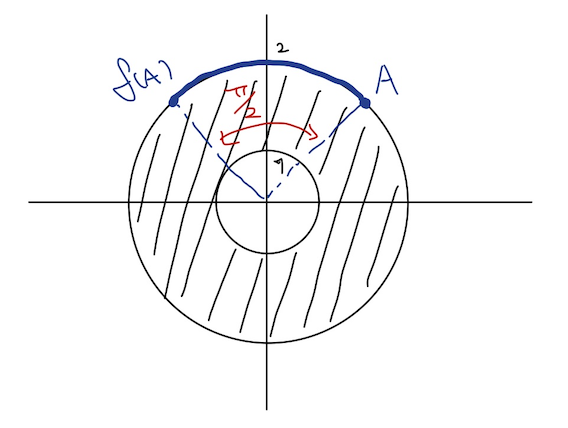
\includegraphics[scale=0.5]{Images/1.png}}
}

\dfn[]{Hyperplane}{
    Hyperplane in $\bbR^n$ is a plane of dimension $n-1$ that divides $\bbR^n$ into semi planes.
}
\begin{itemize}
    \item Hyperplane in $\bbR^1$ is a point.\\
        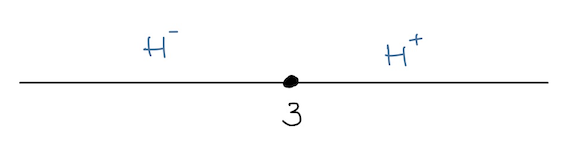
\includegraphics[scale=0.4]{Images/2.png}
    \item Hyperplane in $\bbR^2$ is a line that divides the plane into two half-planes.\\
        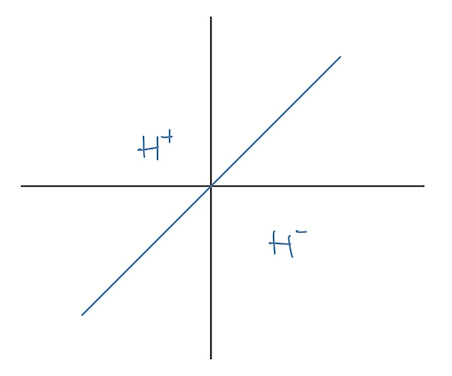
\includegraphics[scale=0.4]{Images/3.png}
    \item Hyperplane in $\bbR^3$ is a plane that divides the space into two half-spaces.\\
        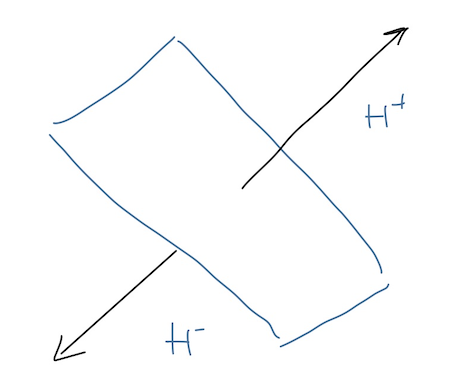
\includegraphics[scale=0.4]{Images/4.png}
\end{itemize}
\thm[]{Hyperplane theorem}{
    If
    \begin{itemize}
        \item $A, B \subset \bbR^n$
        \item $A, B$ disjoint and convex
    \end{itemize}
    then $A,B$ can be separated by a hyperplane.
}
\ex[]{Hyperplane}{
    Separated by a line. 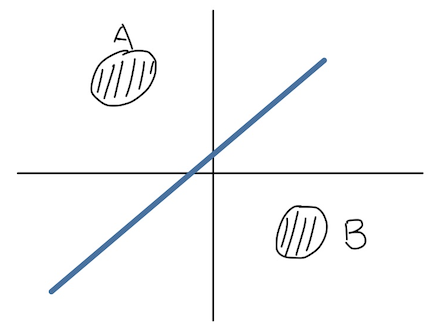
\includegraphics[scale=0.5]{Images/5.png}
}
\ex[]{Hyperplane}{
    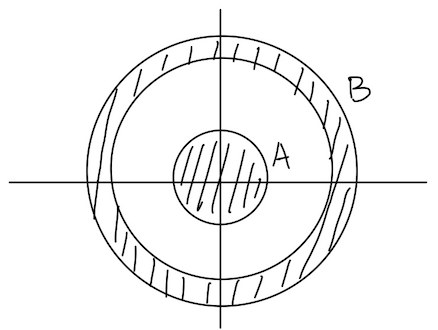
\includegraphics[scale=0.5]{Images/6.png}\\
    Separation theorem cannot be applied because B is not convex.
}

\dfn[]{Correspondence}{
    $A, B$ sets $\subseteq\bbR$\\
    $f: A\to B$ map\\
    $F: A \rightrightarrows B$\\
    $\{(x, F(x)), x \in A, F(x) \subset B\}$\\
    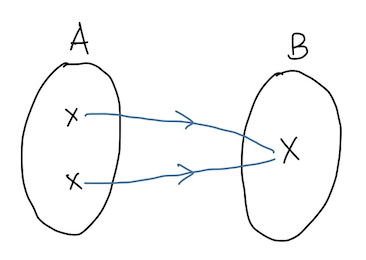
\includegraphics[scale=0.3]{Images/7.png}
}

\ex[]{Corrrespondence}{
    $F: \bbR \rightrightarrows \bbR$\\

    $x \to \begin{cases}
        [1,3] & x\leq 1\\
        \{2\} & x>1
    \end{cases}$\\
    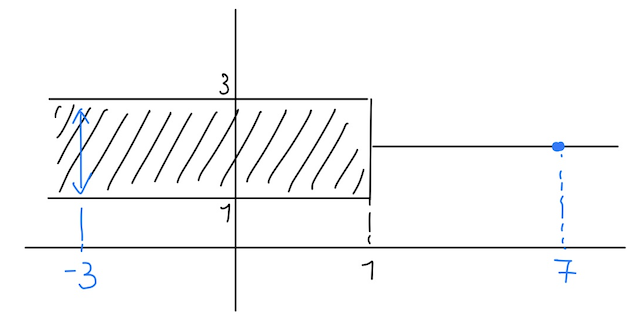
\includegraphics[scale=0.5]{Images/8.png}\\
    $F(\{7\}) = \{2\}$\\
    $F(\{-3\}) = [1,3]$
}
\ex[]{Correspondence}{
    $G: \bbR \rightrightarrows \bbR$\\

    $G(x) = \begin{cases}
        [x-7, x-5] & x<0\\
        (6,9) & x=0\\
        (x+7, x+8] & x>0
    \end{cases}$\bigskip\\

    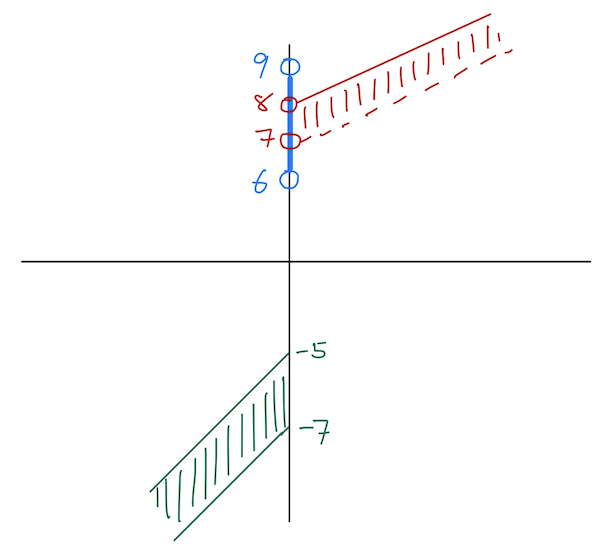
\includegraphics[scale=0.5]{Images/9.png}
}
\ex[]{Correspondence}{
    $f: [0,1]\rightrightarrows[0,1]$\\

    $x\to \begin{cases}
        [0,1] & x=0\\
        \{\frac{1}{2}\} & 0<x<1\\
        [0,\frac{1}{2}] & x = 1
    \end{cases}$\bigskip\\
    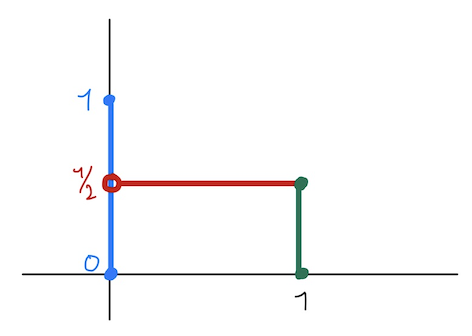
\includegraphics[scale=0.5]{Images/10.png}
}
\ex[]{Correspondence}{
    Important for confidence interval construction of financial data.\bigskip\\
    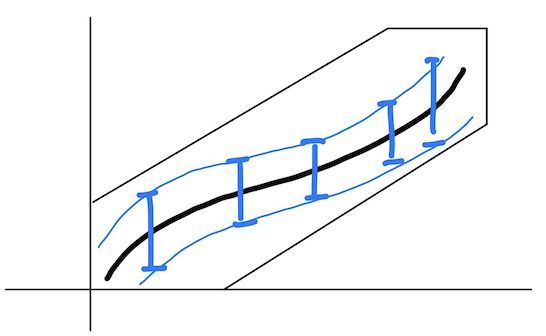
\includegraphics[scale=0.5]{Images/11.png}
}

\dfn[]{Closed graph property}{
    $F: A \rightrightarrows B$ a correspondence, $x\in A$.\\
    
    We say that $F$ has the closed graph property at $x$ if for any converging sequence $(x_n,y_n)_n$ of element in the graph $F$,
    its limit belongs to the graph of $F$.\\
    We say that $F$ has the closed graph property if it has the property above for all $x\in A$.
}
\ex[]{Closed graph property}{
    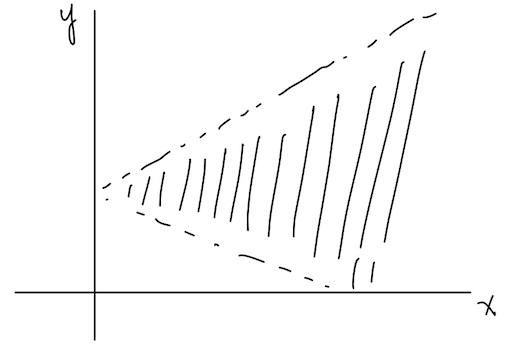
\includegraphics[scale=0.5]{Images/12.png}\\

    F does not have the closed graph property because the graph of F is not closed.
}
\textbf{Proposition: }$F: A\rightrightarrows B$ correspondence. If graph $F$ is \textbf{compact}, then $F$ has the closed graph property.\\


$f: \bbR\to\bbR, x\to f(x)$. $f$ is continuous at $x=a\in\bbR$, if and only if $\lim_{x\to a}f(x)=f(a)$.
Equivalently, $f$ is continuous at $x=a$ if and only if for any open set $u$ containing $f(a)$, $f^{-1}(u)$ is an open set containg $a$.
\ex[]{Continuity}{
    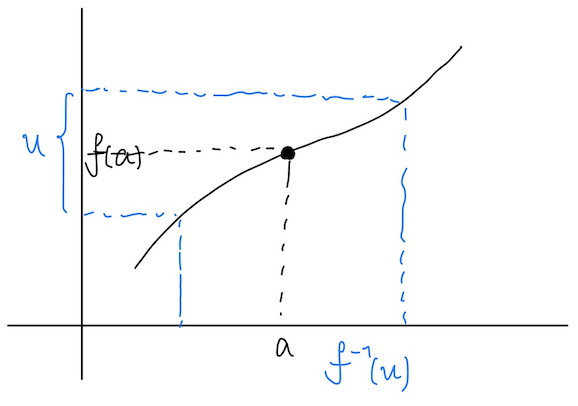
\includegraphics[scale=0.5]{Images/13.png}
}
\ex[]{Continuity}{
    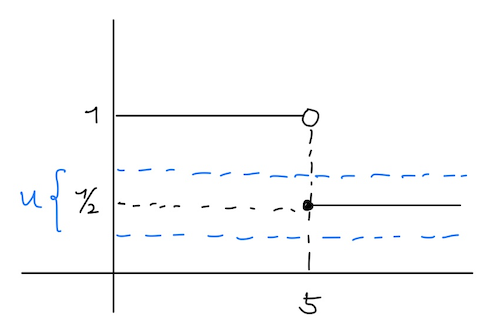
\includegraphics[scale=0.5]{Images/14.png}
    $u$ open set containing $f(5)=\frac{1}{2}$, $f^{-1}(u)=[5,\infty)$ is not an open set containing 5.
}
We are now going to generalize the notion of continuity for correspondence.
\dfn[]{Hemi-continuity}{
    $A, B \subseteq\bbR, a\in A$\\
    $F: A\rightrightarrows B$ is a correspondence\\

    We say that $F$ is upper hemi-continuous at $x=a$ if for all open set $u$ containing $f(a)$, 
    its pre-image $F^{-1}(u)$ is an open set containing a.
    The correspondence $F$ is upper hemi-continuous if the above property holds for every $a\in A$.
}
\ex[]{Hemi-continuity}{
    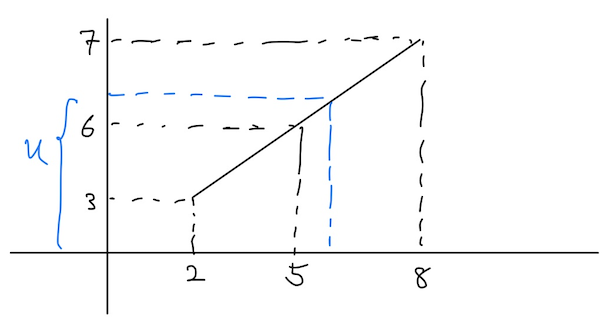
\includegraphics[scale=0.5]{Images/15.png}\\

    $f(\{5\})=[0,6]$\\
    $f$ is upper hemi-continuous.
}
\ex[]{Hemi-continuity}{
    $f: [0,1]\rightrightarrows [0,1]$\\

    $x\to 
    \begin{cases}
        [0,1] & x\neq\frac{1}{2}\\
        \frac{1}{2} & x=\frac{1}{2}
    \end{cases}$\bigskip\\

    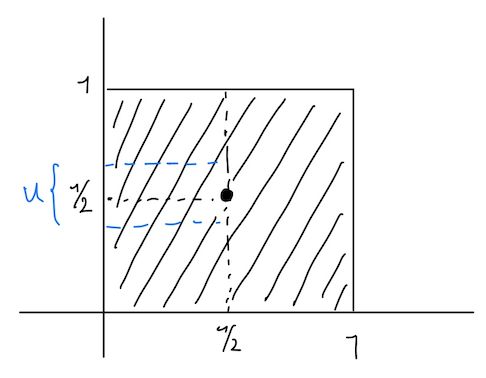
\includegraphics[scale=0.5]{Images/16.png}\\

    $u$ open set containing $f(\frac{1}{2})=\frac{1}{2}$\\
    $f^{-1}(u) = \{\frac{1}{2}\}$ is not an open set. $\Rightarrow$ $f$ is not hemi-continuous.
}

\thm[]{Kakutani fixed point theorem}{
    \begin{itemize}
        \item $A, B \subseteq\bbR^n \text{ convex and compact}$
        \item $F: A\rightrightarrows B$
    \end{itemize}
    If
    \begin{enumerate}
        \item $F$ is upper hemi-continuous
        \item $F(x)$ is convex, $\forall x\in A$
    \end{enumerate}
    then $F$ has at least one fixed point.
}
\textbf{Remark:}
\begin{itemize}
    \item This theorem is a generalization of the Brouwer fixed point theorem.
    \item The second property of Kakutani fixed point theorem means that correpondence cannot have the follwing behavior\bigskip\\
        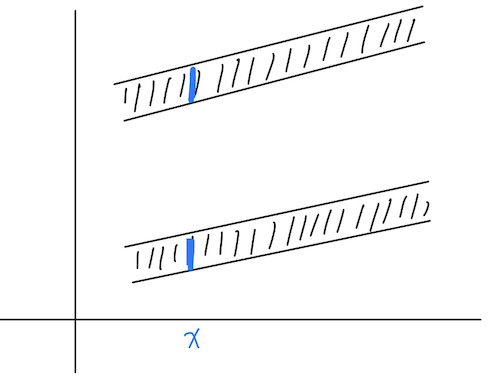
\includegraphics[scale=0.4]{Images/17.png}
\end{itemize}
\ex[]{Kakutani}{
    $F: [0,2]\rightrightarrows [0,2]$\\

    $x\to
    \begin{cases}
        \{1\} & 0\leq x<1\\
        [1,2] & x=1\\
        \{2\} & 1<x\leq 2
    \end{cases}$\bigskip\\

    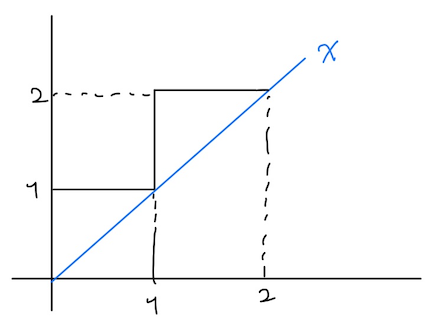
\includegraphics[scale=0.5]{Images/18.png}\\
    
    Fix $F = \{1,2\}$
}
\ex[]{Kakutani}{
    $F: [0,20]\rightrightarrows [0,20]$\\

    $x\to
    \begin{cases}
        10-x & 0\leq x<7\\
        [3,20] & x=7\\
        x-4 & 7<x\leq 20
    \end{cases}$\bigskip\\

    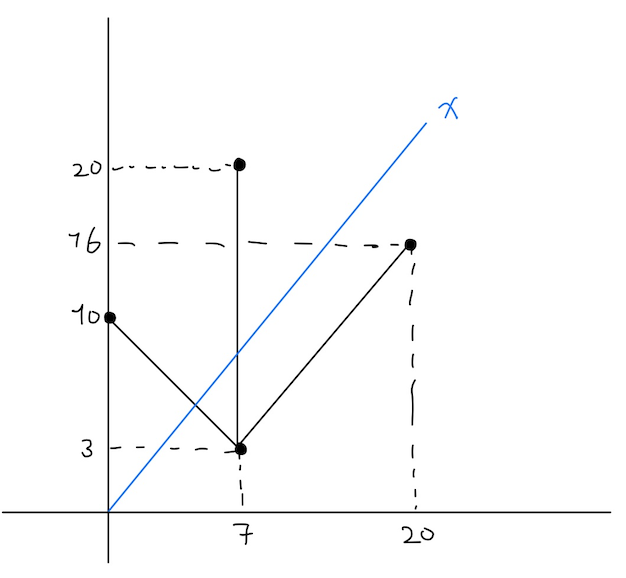
\includegraphics[scale=0.5]{Images/19.png}\\

    $10 - x = x \leftrightarrow x=5$\\
    $F$ is a fixed point because $\{F\}\subset F(\{7\})$\\
    Fix $F = \{5,7\}$
}

Hemi-continuous is hard to prove for the Kakutani theorem, thus we have the following \textbf{proposition}:
$F: A\rightrightarrows B$ correspondence. 
If $F$ has the closed graph property, then $F$ is upper hemi-continuous.
The scheme is as the following: Graph $F$ is compact $\Rightarrow$ Graph $F$ has the closed graph property $\Rightarrow$ $F$ is upper hemi-continous.

\section{What is necessary to know in this chapter?}
\begin{enumerate}
    \item Functions, sequences, cardinality, continuity
    \item Typology in $\bbR^n$
    \item Hyperplane separation theorem
    \item Weierstrass theorem
    \item Intermediate value theorem
    \item Banach fixed point theorem
    \item Brouwer fixed point theorem
    \item Kakutani fixed point theorem
\end{enumerate}

%\dfn{Definition Topic}{Definition Statement}
%\thm{Theorem Name}{Theorem Statement}
%\cor[cori]{Corollary Name}{Corollary Statement}
%\lem{Lemma Name}{Lemma Statement}
%\clm{Claim Name}{Claim Statement}
%\ex{Example Name}{Example explained}
%\opn{Open Question Name}{Question Statement}
%\pr{Question Name}{Question Statement}
%\nt{Special Note}
%\wc{Wrong Concept topic}{Explanation}
%\proof{Proof Idea}{}